%\renewcommand{\thefigure}{\theenumi}
%\renewcommand{\thetable}{\theenumi}
\renewcommand{\theequation}{\theenumi}
\begin{enumerate}[label=\thesection.\arabic*.,ref=\thesection.\theenumi]
\numberwithin{equation}{enumi}
\numberwithin{table}{enumi}


\item Two dice, one blue and one grey, are thrown at the same time.  
\begin{enumerate}
\item  Complete Table \ref{table:1.2.133}.
\item  A student argues that there are 11 possible outcomes 2, 3, 4, 5, 6, 7, 8, 9, 10, 11 and 12. Therefore, each of them has a probability $\frac{1}{11}$. Do you agree with this argument? Justify your answer.
\end{enumerate}
%
\begin{table}[ht!]
\centering
\input{./solutions/10-1/prob/codes/tables/input.tex}
\caption{Input Values}
\label{table:1.2.133}	
\end{table}
\item A die is thrown once. Find the probability of getting\\
(i) a prime number;\\
(ii) a number lying between 2 and 6;\\
(iii) an odd number.
\\
\solution
In general, the complex number $\myvec{a_1\\a_2}$ has the matrix representation
\begin{align}
\label{eq:3.4.1_Complex}
\myvec{a_1\\a_2} &= \myvec{a_1 & -a_2\\ a_2 & a_1}\myvec{1\\0}
\\
&= \vec{T}_a\myvec{1\\0}
\\
\implies \myvec{5\\-3}&=\myvec{5&3\\-3&5}\myvec{1\\0}
\end{align}
Then,
\begin{align}
\myvec{5\\-3}^3 &\triangleq\myvec{5&3\\-3&5}^3\myvec{1\\0}
\\
 &= \myvec{-10&198\\-198&-10} \myvec{1\\0}
\\
&=\myvec{-10\\-198}
\end{align}
The python code for above problem is
\begin{lstlisting}
codes/line/comp.py
\end{lstlisting}

\item In a game, a man wins a rupee for a six and loses a rupee for any other number when a fair die is thrown. The man decided to throw a die thrice but to quit as and when he gets a six. Find the expected value of the amount he wins / loses.\\
\item 
\item Find the probability of getting 5 exactly twice in 7 throws of a die.\\
\solution
\input{solutions/4/4.5.tex}

\item 

\item
\item 
\item Let X denote the sum of the numbers obtained when two fair dice are rolled. Find the variance and standard deviation of X.\\
\solution
When two fare dice are rolled. The sum of the numbers obtained can have the values 2, 3, 4, 5, 6, 7, 8, 9, 10, 11, 12.\\
$\pr{X}$ = probability of obtaining X as the sum and let us represent the case when first dice shows the number $x_1$ and the second dice shows the number $x_2$ as $(x_1,x_2)$.
\begin{table}[hbt!]
\resizebox{\columnwidth}{!}{
\begin{tabular}{|l|c|c|c|c|c|c|c|c|c|c|c|}
\hline
\multicolumn{1}{|c|}{x} & 2 & 3 & 4 & 5 & 6 & 7 & 8 & 9 & 10 & 11 & 12 \\ \hline
$\pr{X}$                   &$\frac{1}{36}$   &$\frac{2}{36}$   &$\frac{3}{36}$   &$\frac{4}{36}$   &$\frac{5}{36}$   &$\frac{6}{36}$   &$\frac{5}{36}$   &$\frac{4}{36}$   &$\frac{3}{36}$    &$\frac{2}{36}$    &$\frac{1}{36}$    \\ \hline
\end{tabular}
}
\caption{Probability Distribution Table of X}
\label{table:1}
\end{table}
For the above problem,we know that.
\begin{align}
p_x\brak{n} &= 
  \begin{cases}
    0 & \text{if } n \leq 1,\\
    \frac{n-1}{36} & \text{if } 2 \leq n \leq 7,\\
    \frac{13-n}{36} & \text{if } 7 < n \leq 12,\\
    0 & \text{if } n>12.
  \end{cases}
\end{align}
\begin{align}
    &Mean,E(X) \nonumber\\
    & =\sum_{k=1}^{12} (k \times p_x\brak{k})\\
    & = \sum_{k=1}^{6}k\times\frac{1}{36}[k-1] + \sum_{k=7}^{12}k\times\frac{1}{36}[13-k]\\
    & = \frac{1}{36}\left[\sum_{k=1}^{6}k(k-1) + \sum_{k=7-6}^{12-6}(k+6)\times[13-(k+6)]\right]\\
    & = \frac{1}{36}\left[\sum_{k=1}^{6}k(k-1) + \sum_{k=1}^{6}(k+6)\times[13-(k+6)]\right]\\
    &= \frac{1}{36}\sum_{k=1}^{6}\left(k(k-1) + (k+6)(7-k)\right)\\
    &= \frac{1}{36}\sum_{k=1}^{6}\left((k^2- k)+ (7k-k^2+42-6k)\right)\\
    &= \frac{1}{36}\sum_{k=1}^{6}\left( 42\right)\\
    &= \frac{1}{36}\left[ 42 \times 6 \right]
\end{align}
Therefore,
 Mean, $E\brak{X} = 7$
 
\begin{align}
  Variance,\sigma^2 &= E\brak{X-E\brak{X}}^2 \\
    &= E\brak{X^2} - \brak{E\brak{X}}^2
\end{align}
Let us consider $E\brak{X^2}$,
\begin{align}
    & E\brak{X^2} \nonumber\\
    &= \left(\sum_{k=1}^{12}(k^2\times p_x(k))\right)\\
    &= \sum_{k=1}^{6}k^2\times\frac{1}{36}[k-1] + 
    \sum_{k=7}^{12}(k)^2\times[13-k]\\
    &\text{by rearrangement we get}\\
    &= \frac{1}{36}\left[\sum_{k=1}^{6}k^2(k-1) + \sum_{k=7-6}^{12-6}(k+6)^2\times[13-(k+6)]\right]\\
    &= \frac{1}{36}\left[\sum_{k=1}^{6}k^2(k-1) + \sum_{k=1}^{6}(k+6)^2(7-k)\right]\\
    &= \frac{1}{36}\sum_{k=1}^{6}\left(k^2(k-1) + (k^2+36+12k)(7-k)\right)\\
    &= \frac{1}{36}\sum_{k=1}^{6}\left((k^3-k^2) + (-k^3-5k^2+48k+252)\right)\\
    &= \frac{1}{36}\sum_{k=1}^{6}(-6k^2+48k+252)\\
    &= \frac{1}{6}\sum_{k=1}^{6}(-k^2+8k+42)\\
    &= \frac{1}{6}\left[ -\frac{(6)(7)(13)}{6} + 8\times\frac{(6)(7)}{2}+ (42)(6) \right]\\
    &= \frac{1}{6}[-91+168+252]\\
    &= \frac{329}{6}
\end{align}

\begin{align}
    \text{ Variance, }\sigma^2 &=E\brak{X^2} - \brak{E\brak{X}}^2\\
    &= \frac{329}{6}- ((7)^2)\\
    &= \frac{329}{6} - 49\\
   \sigma^2 &= \frac{35}{6}
\end{align}
%
\item Two numbers are selected at random (without replacement) from the first six positive integers. Let X denote the larger of the two numbers obtained. Find E(X).\\
%
\solution
\input{solutions/4/4.10.tex}
\item
\item Determine P(E/F), if a die is thrown three times,\\
E : 4 appears on the third toss, F : 6 and 5 appears respectively on first two tosses\\

\item In a musical chair game, the person playing the music has been
advised to stop playing the music at any time within 2 minutes after she starts playing.What is the probability that the music will stop within the first half-minute after starting?
\solution
Let the random variable  $X\in\mathbb{R^+} $ represent the time between starting the music and stopping in minutes
For a uniform probability distribution, the Probability Density Function(pdf) is given by
\begin{align}
  p_{X}(x) =
  \begin{cases}
  \dfrac{1}{b-a} = \dfrac{1}{2} & \text{if $0 \leq x \leq 2$}\\ \vspace{-0.1cm}
  0 & \text{otherwise} 
  \end{cases}
\end{align}
The probability that the music will stop within the first half-minute after starting
\begin{align}
    \pr{X=x \,\,|\,\, 0 \leq x \leq 0.5} = \int_0^{\frac{1}{2}} \frac{1}{2} dx = \frac{1}{4} =0.25
\end{align}
\item A missing helicopter is reported to have crashed somewhere in the rectangular region shown in Fig. 15.2. What is the probability that it crashed inside the
lake shown in the figure?
\begin{figure}[!ht]
\centering
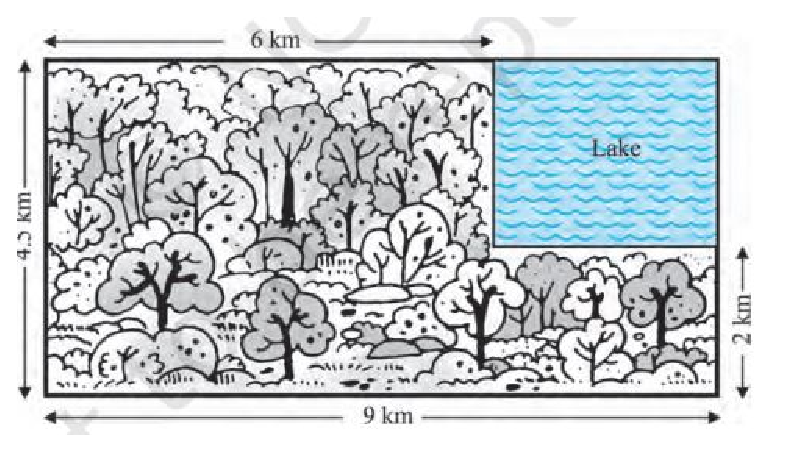
\includegraphics[width=\columnwidth]{./prob/figs/lake.eps}
\caption{}
\label{fig:lake}
\end{figure}
\solution
\input{solutions/4/4.14.tex}

   \item On one page of a telephone directory, there were 200 telephone numbers.
The frequency distribution of their unit place digit (for example, in the number 25828573, the unit place digit is 3) is given in Table \ref{table:prob_exam4}
below

\begin{table}[!ht]
\centering
\resizebox{\columnwidth}{!}{
\begin{tabular}{ |c|c|c|c|c|c|c|c|c|c|c| } 
\hline
 \textbf{Digit} &0 &1 &2 &3 &4 &5 &6 &7 &8 &9 \\ 
 \hline
 \textbf{Frequency} &22 &26 &22 &22 &20 &10 &14 &28 &16 &20 \\ 
 \hline
\end{tabular}
}
\caption{}
\label{table:prob_exam4}
\end{table}
Without looking at the page, the pencil is placed on one of these numbers, i.e., the number is chosen at random. What is the probability that the digit in its unit place is 6?\\
\solution
In general, the complex number $\myvec{a_1\\a_2}$ has the matrix representation
\begin{align}
\label{eq:3.4.1_Complex}
\myvec{a_1\\a_2} &= \myvec{a_1 & -a_2\\ a_2 & a_1}\myvec{1\\0}
\\
&= \vec{T}_a\myvec{1\\0}
\\
\implies \myvec{5\\-3}&=\myvec{5&3\\-3&5}\myvec{1\\0}
\end{align}
Then,
\begin{align}
\myvec{5\\-3}^3 &\triangleq\myvec{5&3\\-3&5}^3\myvec{1\\0}
\\
 &= \myvec{-10&198\\-198&-10} \myvec{1\\0}
\\
&=\myvec{-10\\-198}
\end{align}
The python code for above problem is
\begin{lstlisting}
codes/line/comp.py
\end{lstlisting}


\item Suppose we throw a die once. (i) What is the probability of getting a number greater than 4 ? (ii) What is the probability of getting a number less than or
equal to 4 ?
\\
\solution
In general, the complex number $\myvec{a_1\\a_2}$ has the matrix representation
\begin{align}
\label{eq:3.4.1_Complex}
\myvec{a_1\\a_2} &= \myvec{a_1 & -a_2\\ a_2 & a_1}\myvec{1\\0}
\\
&= \vec{T}_a\myvec{1\\0}
\\
\implies \myvec{5\\-3}&=\myvec{5&3\\-3&5}\myvec{1\\0}
\end{align}
Then,
\begin{align}
\myvec{5\\-3}^3 &\triangleq\myvec{5&3\\-3&5}^3\myvec{1\\0}
\\
 &= \myvec{-10&198\\-198&-10} \myvec{1\\0}
\\
&=\myvec{-10\\-198}
\end{align}
The python code for above problem is
\begin{lstlisting}
codes/line/comp.py
\end{lstlisting}

\item  Given that the two numbers appearing on throwing two dice are different. Find the probability of the event `the sum of numbers on the dice is 4'.\\
\solution

	 Given the production yield per hectare of wheat of 100 farms of a village. 
		The following python code generates the required ogive.
	\begin{lstlisting}
	./solutions/20-30/codes/statistics/exercises/q25.py
	\end{lstlisting}


	
	\begin{figure}[!ht]
	\centering
	\includegraphics[width=\columnwidth]{./solutions/20-30/figs/statistics/exercises/ex_q25.eps}
	\caption{}
	\label{fig:q25_ogive}	
	\end{figure}
	
	\begin{table}[ht]
	%\begin{center}
    	\input{./solutions/20-30/tables/statistics/exercises/stat_ex_q25_ans.tex}
	\caption{production yield using more than cumulative frequency}
	\label{table:stat_ex_q25anstable4}
	%\end{center}
	\end{table}




\item A game of chance consists of spinning an arrow which comes to rest pointing at one of the numbers 1, 2, 3, 4, 5, 6, 7, 8 (see Fig. \ref{fig:122} ), and these are equally likely outcomes. What is the probability that it will point at\\
(i) 8 ?\\
(ii) an odd number?\\
(iii) a number greater than 2?\\
(iv) a number less than 9?\\
\begin{figure}[!ht]
\centering

\includegraphics[width=\columnwidth]{./prob/figs/clock.eps}
\caption{}
\label{fig:122}
\end{figure}
\\
\solution
In general, the complex number $\myvec{a_1\\a_2}$ has the matrix representation
\begin{align}
\label{eq:3.4.1_Complex}
\myvec{a_1\\a_2} &= \myvec{a_1 & -a_2\\ a_2 & a_1}\myvec{1\\0}
\\
&= \vec{T}_a\myvec{1\\0}
\\
\implies \myvec{5\\-3}&=\myvec{5&3\\-3&5}\myvec{1\\0}
\end{align}
Then,
\begin{align}
\myvec{5\\-3}^3 &\triangleq\myvec{5&3\\-3&5}^3\myvec{1\\0}
\\
 &= \myvec{-10&198\\-198&-10} \myvec{1\\0}
\\
&=\myvec{-10\\-198}
\end{align}
The python code for above problem is
\begin{lstlisting}
codes/line/comp.py
\end{lstlisting}


\item Find the variance of the number obtained on a throw of an unbiased die.
\solution
%Let $X \in \{1,2,3,4,5,6\}$, be the random variable representing outcome of the die.The probability mass function(pmf) can be expressed as
\begin{align}
p_X\brak{n} = P\brak{X=n} =  \begin{cases}
			\frac{1}{6}, & \text{if $1 \leq n\leq 6$}\\
            0, & \text{otherwise}
		 \end{cases} 
\end{align}



		              
The variance (Var(X)) of this distribution can be found by definition,\\
\begin{align}
Var\brak{X} = E\brak{X^{2}}-\brak{E\brak{X}}^{2} \label{Eq:5.30:1}
\end{align}
where,
\begin{align}
E\brak{X}=\sum_{k=1}^{k=6} kp_X\brak{k}  \\
E\brak{X}=\frac{1}{6}\sum_{k=1}^{k=6} k \label{Eq:5.30:2}
\end{align}
We know that, sum of natural numbers from 1 to n is,
\begin{align}
\sum_{k=1}^{k=n} k = \frac{n\brak{n+1}}{2} \label{Eq:5.30:3}
\end{align}
By substituting the formula from \eqref{Eq:5.30:3} in \eqref{Eq:5.30:2} and n=6, We get,
\begin{align}
E\brak{X}=\frac{1}{6} \times \frac{6\times7}{2}  \\
E\brak{X}=\frac{7}{2} \label{Eq:5.30:4}
\end{align}
And,
\begin{align}
E\brak{X^{2}}=\sum_{k=1}^{k=6} k^{2}p_X\brak{k}  \\
E\brak{X^{2}}=\frac{1}{6}\sum_{k=1}^{k=6} k^{2} \label{Eq:5.30:5}
\end{align}
We know that, sum of squares of natural numbers from 1 to n is,
\begin{align}
\sum_{k=1}^{k=n} k^{2} = \frac{n\brak{n+1}\brak{2n+1}}{6} \label{Eq:5.30:6}
\end{align}
By substituting the formula from \eqref{Eq:5.30:6} in \eqref{Eq:5.30:5} and n=6, We get,
\begin{align}
E\brak{X^{2}}=\frac{1}{6} \times \frac{6\times7\times13}{6}  \\
E\brak{X^{2}}=\frac{91}{6} \label{Eq:5.30:7}
\end{align}
By substituting the values from \eqref{Eq:5.30:7} and \eqref{Eq:5.30:4} in \eqref{Eq:5.30:1}
\begin{align}
Var\brak{X} = E\brak{X^{2}}-\brak{E(X)}^{2}  \\
Var\brak{X} = \frac{91}{6} - \frac{49}{4}  \\
Var\brak{X} = \frac{70}{12}  \\
Var\brak{X} = 2.9167 \label{Eq:5.30:8}
\end{align}
\end{enumerate}


